\subsection{Is DC a Feasible Alternative to AC in Commercial Lighting Systems?}

This section to answer the overall question of the project. The previous four questions will be summarised and the information combined to form an overall design conclusion.
 
\subsubsection{Assumptions} \label{section:sam-assumptions}

%New Paragraph
The following assumptions have been made to propose a design:

\begin{itemize}[noitemsep,nolistsep]
	\item Location is Brisbane, Queensland, Australia
	\item PV tilt at Brisbane's latitude of 27 degrees
	\item Specified modules are the Suntech 265W monocrystalline \cite{website:SuntechModule2}
	\item Ground Coverage Ratio of 0.5
	\item QUT P Block is an accurate test case for building scaling
\end{itemize}

\subsubsection{Building Energy Specifications}

\paragraph{Maximum Lighting Demand}
~\\
%New Paragraph
As previously analysed in Section \ref{section:question3}, a simple office room was modelled with lighting requirements based on QUT P\,Block. The table from this section is reproduced below in Table \ref{table:QUTlvl7-count2}. The total loads are from a full corporate building level.    

\begin{table}[!ht]
	\centering
	\renewcommand{\arraystretch}{2}
	\begin{tabular}{|c|c|c|c|c|}
		\hline
		\textbf{Fitting} & \textbf{Wattage (W)} & \textbf{Voltage (V)} & \textbf{Count} & \textbf{Demand (A)} \\ \hline
		2 x 18W Fluorescent & 18.0 & 230.0 & 220 &  0.08 \& 17.2 \\ \hline
		2 x 28W Fluorescent & 28.0 & 230.0 & 448 & 0.12 \& 54.5 \\ \hline
	\end{tabular}
	
	\caption{QUT: P Block Level 7 Lighting Count and Calculations}
	\label{table:QUTlvl7-count2}
\end{table} 

\begin{figure}[H]
	\hfill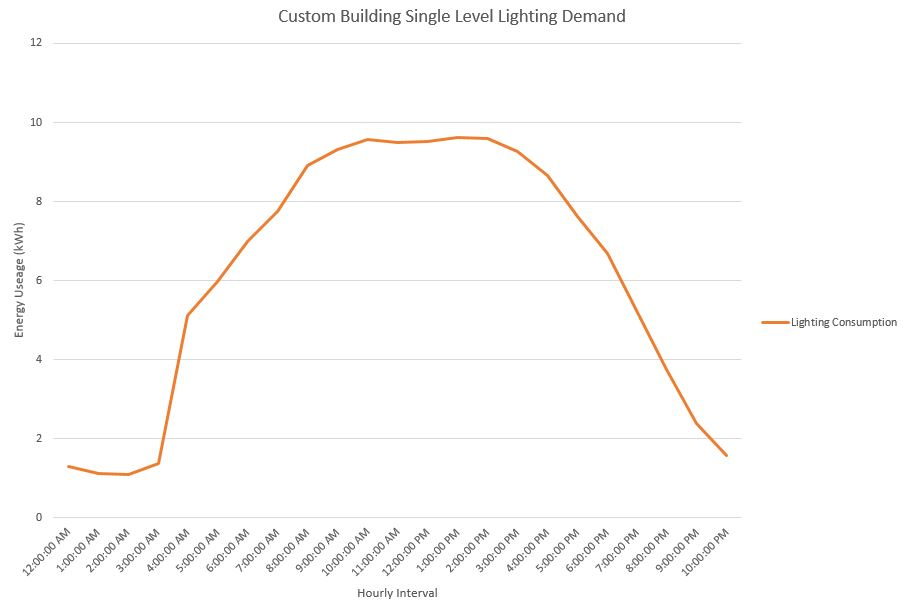
\includegraphics[width = 150mm]{images/custom-building/lighting-demand}\hspace*{\fill}
	\caption{Custom Building: Predicted Single Level Lighting Demand} 
	\label{fig:custom-building-lighting-demand}
\end{figure}

%New Paragraph
Figure \ref{fig:custom-building-lighting-demand} shows the predicted lighting energy demand in kilowatt hours. This curve can be used to size the photovoltaic array required for one level. 

\paragraph{Required Photovoltaic Array}
~\\
%New Paragraph
Over a year, the metering data shows that there will be 42,243\,kWh of single level lighting consumption. In order to supply enough energy to power the lighting for one of the proposed levels, the array must produce a minimum of 42,243\,kWh per year with the production curves ideally fitting the consumption curves to ensure that the connection to the grid is unnecessary. Utilising the assumptions stated in Section \ref{section:sam-assumptions}, an array was modelling that could produce the required electricity. Again, using System Model Advisor, 44,047\,kWh\,DC/Year will be produced with 95 modules from 5 strings of 19 modules.

\begin{table}[H]
	\centering
	\begin{tabular}{|l|c|}
		\hline
		\textbf{Design Variable} & \multicolumn{1}{l|}{\textbf{Value}} \\ \hline
		Nameplate Capacity & 25.21\,kW \\ \hline
		Number of Modules & 95 \\ \hline
		Modules Per String & 19 \\ \hline
		Strings in Parallel & 5 \\ \hline
		Module Area & 154.6\,\si{m^2} \\ \hline
		Annual DC Energy & 44,047.4\,kWh/yr \\ \hline
	\end{tabular}
	\caption{Custom Building: Single Level Array Design Table}
	\label{table:custom-building}
\end{table} 

%New Paragraph
To calculate the required array for this array, the equation from Section \ref{section:mounting-panels} can be utilised. This considers the assumed spacings between modules to allow for an accurate estimation of the total area required. 

\begin{center}
	\textit{Total Required Area = Module Area / GCR + Laneway Allowance}
	\newline
	Total Required Area = 154.6 / 0.5 + 5\%
	\newline
	Total Required Area = 325\,\si{m^2}
\end{center} 

%New Paragraph
This calculation allows their to be the conclusion that to power one level of a commercial building, 325\,\si{m^2} will be required on the building's roof for PV mounting. 

\paragraph{Demand vs Production Curve}
~\\
%New Paragraph
The next stage of the feasibility study is whether the consumption vs production curve of energy match. In this instance, due to PV producing during daylight the system will not be capable of producing energy at all times consumption is occurring. Figure \ref{fig:custom-building-production-vs-consumption} below represents this situation.  

\begin{figure}[H]
	\hfill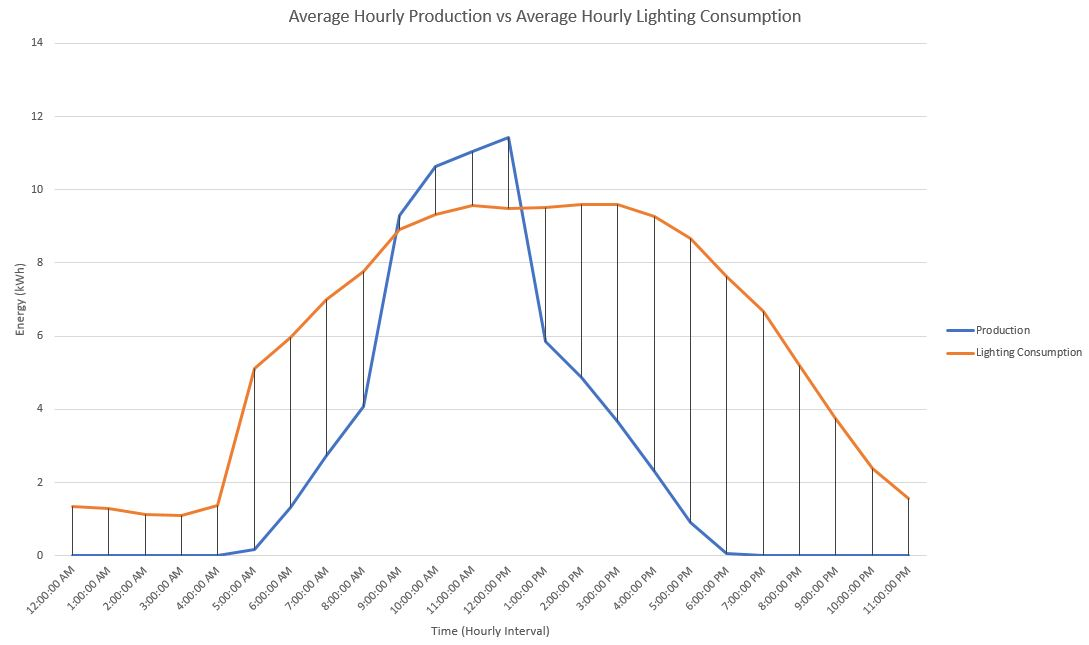
\includegraphics[width = 150mm]{images/custom-building/production-vs-consumption}\hspace*{\fill}
	\caption{Custom Building: Production vs Consumption Curve} 
	\label{fig:custom-building-production-vs-consumption}
\end{figure}  

It should be noted that the modelled system produces enough energy annually but the curves do not match as mentioned previously. This can be explained by the time periods from 9\,AM to 1\,PM that, on average over one year, producing higher than required energy. Due to this, as predicted earlier in the report, a battery is required. At this stage there are a two main design options:

\begin{enumerate} [noitemsep]
	\item Install a battery to discharge from approximately 2\,PM through to 9\,AM the following day
	\item Oversize the system so that 5\,AM through to 5\,PM is covered by immediate production and install a battery for overproduction
	\item Separate from the original proposal and employ a dual connection with two drivers. When no direct DC connection is available, the device switches back to AC 
\end{enumerate} 

The risk with option 1 is that during lower production periods such as winter, the additional production may not be enough to support the darker hours. Since June is a worst case, the system must be modelled to properly perform at this period. Figure \ref{fig:custom-building-production-vs-consumption-best-vs-worst} compares    

\begin{figure}[H]
	\hfill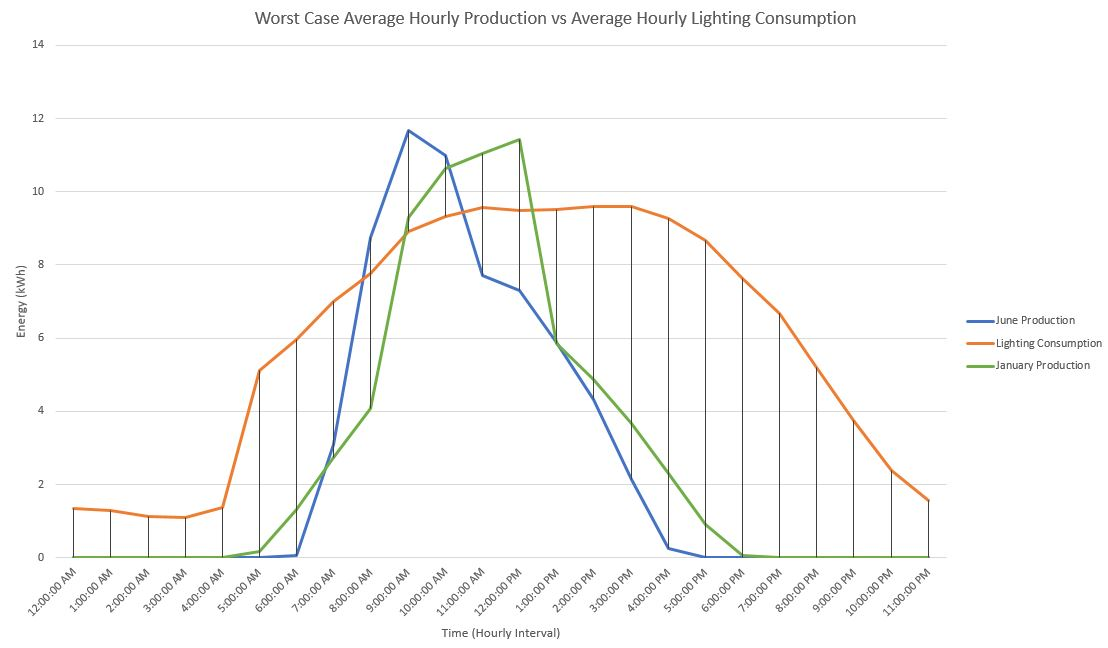
\includegraphics[width = 150mm]{images/custom-building/production-vs-consumption-worst-vs-best-case}\hspace*{\fill}
	\caption{Custom Building: June and January Production vs Consumption Curve} 
	\label{fig:custom-building-production-vs-consumption-best-vs-worst}
\end{figure}  

As seen in Figure \ref{fig:custom-building-production-vs-consumption-best-vs-worst}, the major difference between Summer and Winter appears to be the time shift rather than maximum production. Additionally, as expected the winter production time line has shrunk by one hour either side to 6\,AM to 4\,PM. This conclusion again leads to the conclusion that a small battery will be required on site. Due to altering weather conditions, it is suggested that the system be slightly oversized to allow for poor production periods as the luminaires will not have an AC connection.  

\subsubsection{Efficiency Comparison}

\paragraph{Losses in AC and DC Systems}
~\\
A simple way to model some of the losses of the AC system will be through System Advisor Model that was already created to predict production. These losses are represented in Figure \ref{fig:custom-building-modelled-system-losses}. As can be seen, the losses are separated into soiling and shading, DC losses and AC losses. The total losses for the AC portion of PV modelling is:  

\begin{center}
	PV Array Losses = 4.999 + 7.504 + 1.973 + 0.493 + 1.973 + 0.275 + 0.263 + 0.018 + 2.309 + 1
	\newline
	PV Array Losses = 20.807\%
\end{center} 

\begin{figure}[H]
	\hfill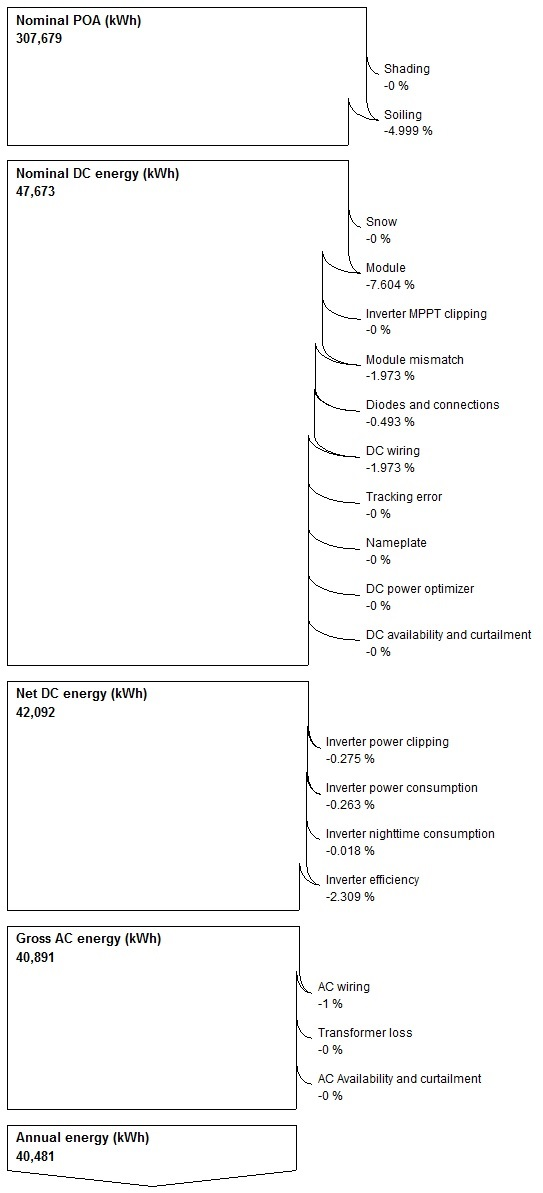
\includegraphics[width = 100mm, height = 220mm]{images/custom-building/sam-losses-265w}\hspace*{\fill}
	\caption{Custom Building: Modelled System Losses} 
	\label{fig:custom-building-modelled-system-losses}
\end{figure}   

Traditional AC system losses will be different due to each separate stage. This includes general cable losses, load losses but more specifically the converter losses. From Figure \ref{fig:custom-building-modelled-system-losses} it can be seen that this accounts for 3.9\% of system losses. To model the comparison, a test system was modelled in Table \ref{table:ac-vs-dc-system-loss-comparison} below. This system compares an AC and DC system with PV production, AC and DC coupled batteries respectively, an assumed 100\,m cable run of 2.5\,\si{mm^2} cable, and an example ballast for LED luminaire. The PV system values were sourced from System Model Advisor. The batteries that were assumed for efficiency values were the Enphase AC battery \cite{website:Enphase-Battery-Data} and the Tesla Powerwall \cite{website:Tesla-Powerwall-Data}. The cable runs were calculated as per Table \ref{table: AC-vs-DC-lengths} and the ballasts were researched to find the average efficiency model.    

\begin{table}[H]
	\centering
	\begin{tabular}{|l|c|c|c|c|}
		\hline
		\multicolumn{5}{|c|}{\textbf{Approximate Energy Losses Modelling AC vs DC}} \\ \hline
		\textbf{Variable} & \multicolumn{1}{l|}{\textbf{AC \%}} & \multicolumn{1}{l|}{\textbf{AC Energy (kWh)}} & \multicolumn{1}{l|}{\textbf{DC \%}} & \multicolumn{1}{l|}{\textbf{DC Energy (kWh)}} \\ \hline
		\textit{PV System} & 20.81\% & 40,481 & 17.00\% & 42,092 \\ \hline
		\textit{Battery} & 4.00\% \cite{website:Enphase-Battery-Data}  & 38,862 & 7.50\% \cite{website:Tesla-Powerwall-Data} & 38,935 \\ \hline
		\textit{100m Cable Run} & 0.96\% & 38,489 & 4.79\% & 37,070 \\ \hline
		\textit{Ballast} & 15.00\% \cite{website:AussieLightingCouncil} & 32,715 & 3.00\% \cite{website:LED-DC-DC-Driver} & 35,958 \\ \hline
		\textit{Total Loss} & \multicolumn{2}{c|}{19.18\%} & \multicolumn{2}{c|}{14.57\%} \\ \hline
	\end{tabular}
	\caption{Approximate Energy Losses Modelling for AC vs DC}
	\label{table:ac-vs-dc-system-loss-comparison}
\end{table} 
 
\paragraph{Losses Discussion}
~\\
Provided that the assumptions made to calculate \ref{table:ac-vs-dc-system-loss-comparison} and the modelling system was accurate, there is a 4.61\% improvement in efficiency by using this proposed, extra-low voltage system. It should be noted that there will be various cable lengths throughout the built system so this can not simply be scaled to the size of the system. Additionally, this calculation was based off one building level however this does not effect the percentage values, only the kWh values.

%New Paragraph 


\subsubsection{Financial Analysis}

% New Paragraph
This section outlines the approximate costs involved with the installation of the proposed extra low voltage DC power distribution system. It should be noted that the expectation is that this system would be installed in a new building. This is due to the expectation that energy cost savings will take a substantial amount of time to break even financially. That is, the additional costs of PV and battery installation will not be recovered from financial benefits from energy savings for a substantial time frame. Due to this, it is unlikely to be financially feasible to remove existing AC infrastructure in place for ELV DC. All financial information should be interpreted as approximations from research and industry experience.     

\paragraph{Luminaire Cost Comparison}
~\\

%New Paragraph
The LED luminaire will accept the same voltage level regardless of whether the upstream power is AC or DC due to the ballast in both instances converting the energy into the correct current type and voltage level. For AC, this would be a ballast converting 230\,V\,AC to 48\,V\,DC and for the proposed ELV 48\,V\,DC there would be no conversion required, only regulation and safety. 
\newline

%New Paragraph
  

\paragraph{New Infrastructure Costs}
~\\
****
\newline
This section is intentionally blank. The report is a work in progress and this part of future works.  

\paragraph{Capital Expenditure}
~\\
****
\newline
This section is intentionally incomplete. The report is a work in progress and this part of future works.  

\begin{itemize}[noitemsep,nolistsep]
	\item Panel Costs
	\item Installation Costs
	\item Battery Costs
	\item Cable Costs
	\item Luminaire cost difference
	\item New infrastructure costs
\end{itemize}

\paragraph{Energy Savings}
~\\
****
\newline
This section is intentionally blank. The report is a work in progress and this part of future works.  

\paragraph{Monthly Costs or Savings}
~\\
****
\newline
This section is intentionally blank. The report is a work in progress and this part of future works.  

\paragraph{Return on Investment}
~\\
****
\newline
This section is intentionally blank. The report is a work in progress and this part of future works.  

\paragraph{Payback Period}
~\\
****
\newline
This section is intentionally blank. The report is a work in progress and this part of future works.  

\subsubsection{Finalised Design}

%% Talk about the number of levels and scaled quantities
%% Talk about switchboards and circuit breakers 
%% Mentioned any DC Arcing Stuff

